\documentclass[a4paper,11pt]{amsbook}

\makeatletter
\def\@thm#1#2#3{%
  \ifhmode\unskip\unskip\par\fi
  \normalfont
  \trivlist
  \let\thmheadnl\relax
  \let\thm@swap\@gobble
  \let\thm@indent\indent % indent
  \thm@headfont{\bfseries}% heading font boldface // changed
  \thm@notefont{\fontseries\mddefault\upshape}%
  \thm@headpunct{.}% add period after heading
  \thm@headsep 5\p@ plus\p@ minus\p@\relax
  \thm@space@setup
  #1% style overrides
  \@topsep \thm@preskip               % used by thm head
  \@topsepadd \thm@postskip           % used by \@endparenv
  \def\@tempa{#2}\ifx\@empty\@tempa
    \def\@tempa{\@oparg{\@begintheorem{#3}{}}[]}%
  \else
    \refstepcounter{#2}%
    \def\@tempa{\@oparg{\@begintheorem{#3}{\csname the#2\endcsname}}[]}%
  \fi
  \@tempa
}
\makeatother

\renewcommand{\chaptername}{Lecture}

\usepackage[T1]{fontenc}
\usepackage[latin1]{inputenc}
\usepackage{times}
\usepackage{microtype}
\usepackage{amssymb}
\usepackage{a4wide}
\usepackage{graphicx}
%\usepackage{paralist}
%\usepackage{bbm}
\usepackage{verbatim}
\usepackage{url}

\newcommand{\ba}{{\boldsymbol{a}}}
\newcommand{\balpha}{{\boldsymbol{\alpha}}}
\newcommand{\bb}{{\boldsymbol{b}}}
\newcommand{\bc}{{\boldsymbol{c}}}
\newcommand{\be}{{\boldsymbol{e}}}
\newcommand{\bff}{{\boldsymbol{f}}}
\newcommand{\bnu}{{\boldsymbol{\nu}}}
\newcommand{\bm}{{\boldsymbol{m}}}
\newcommand{\bo}{{\boldsymbol{0}}}
\newcommand{\bp}{{\boldsymbol{p}}}
\newcommand{\bq}{{\boldsymbol{q}}}
\newcommand{\br}{{\boldsymbol{r}}}
\newcommand{\bsigma}{{\boldsymbol{\sigma}}}
\newcommand{\bt}{{\boldsymbol{t}}}
\newcommand{\bv}{{\boldsymbol{v}}}
\newcommand{\bw}{{\boldsymbol{w}}}
\newcommand{\bx}{{\boldsymbol{x}}}
\newcommand{\by}{{\boldsymbol{y}}}
\newcommand{\bz}{{\boldsymbol{z}}}
\newcommand{\bone}{{\boldsymbol{1}}}

\newcommand{\RR}{\mathbb{R}}
\newcommand{\Rgeo}{{\mathbb{R}_{\ge0}}}
\newcommand{\Zgeo}{{\mathbb{Z}_{\ge0}}}
\newcommand{\NN}{\mathbb{N}}
\newcommand{\ZZ}{\mathbb{Z}}
\newcommand{\QQ}{\mathbb{Q}}
\newcommand{\CC}{\mathbb{C}}

\newcommand{\cA}{{\mathcal{A}}}
\newcommand{\cC}{{\mathcal{C}}}
\newcommand{\cD}{{\mathcal{D}}}
\newcommand{\cH}{{\mathcal{H}}}
\newcommand{\cL}{{\mathcal{L}}}
\newcommand{\cO}{{\mathcal{O}}}
\newcommand{\cP}{{\mathcal{P}}}

\newcommand{\scp}[2]{\langle #1,#2\rangle}
\newcommand{\fl}[1]{\left\lfloor #1\right\rfloor}
\newcommand{\ce}[1]{\left\lceil #1\right\rceil}
\newcommand{\rcone}[1]{{{}_\Rgeo\!\left\langle #1\right\rangle}}
\newcommand{\zcone}[1]{{{}_\Zgeo\!\left\langle #1\right\rangle}}

\DeclareMathOperator{\interior}{int}
\DeclareMathOperator{\relint}{relint}
\DeclareMathOperator{\conv}{conv}
\DeclareMathOperator{\cone}{cone}
\DeclareMathOperator{\aff}{aff}
\DeclareMathOperator{\vol}{vol}
\DeclareMathOperator{\dist}{dist}
\DeclareMathOperator{\vertices}{vert}
\DeclareMathOperator{\rang}{rang}
\DeclareMathOperator{\sign}{sign}
\DeclareMathOperator{\pyr}{pyr}
\DeclareMathOperator{\bipyr}{bipyr}
\DeclareMathOperator{\Sl}{Sl}

\DeclareMathOperator{\sgn}{sgn} %signum
\DeclareMathOperator{\ggT}{ggT}

\newcommand{\ojo}[1]{\textsf{\bfseries\boldmath #1}}
\newcommand{\scribe}[1]{\begin{center}\emph{Scribe: #1}\end{center}\bigskip}

\graphicspath{{graphics/}}

\numberwithin{equation}{section}

\newtheorem{theorem}{\textbf{Theorem}}[section]
\newtheorem{lemma}[theorem]{Lemma}
\newtheorem{proposition}[theorem]{Proposition}
\newtheorem{corollary}[theorem]{Corollary}
\newtheorem{conj}[theorem]{Conjecture}
\newtheorem{obs}[theorem]{Observation}
\newtheorem{exercise}[theorem]{Exercise}
\newtheorem{example}[theorem]{Example}
\newtheorem{remark}[theorem]{Remark}

\newtheorem{defn}{\textbf{Definition}}[section]

%\includeonly{lecture2}

\begin{document}

\thispagestyle{empty}

\newcommand{\thisyear}{2013}

\
\vfill
\begin{center}
        \Huge \sffamily\bfseries 
        Discrete and Algorithmic Geometry \thisyear
        \medskip
        (Part 2)

\vspace{2cm}
\LARGE
Julian Pfeifle

\vspace{3cm}

\normalfont\LARGE\sffamily
Version of \today

\vspace{5cm}\
\end{center}

This is the preliminary version of the lecture notes for the second
part of \emph{Discrete and Algorithmic Geometry} (Universitat
Polit�cnica de Catalunya), held in the fall semester of \thisyear\ by Ferran
Hurtado and Julian Pfeifle.

\medskip
These notes are fruit of the collaborative effort of all participating
students, who have taken turns in assembling this text. The name of
each scribe figures in each corresponding section.

\medskip
%The main literature for this course consists of
%\cite{Conway-Sloane-3rd}, \cite{Conway-Strauss08}
%and~\cite{Senechal95}. 

\medskip Suggestions for improvements will always be gladly received
by \texttt{julian.pfeifle@upc.edu}.

\vfill\


% Local Variables: 
% mode: latex
% TeX-master: "dag-upc"
% End: 

\tableofcontents

\chapter{Convex Polytopes}

\scribe{Cecilia Girón}
 
A convexpolytope can be defined in two different ways:
\begin{enumerate}
\item[-] \textit{$V$-polytope} (discrete geometry): is the convex hull of the finite non-empty point set in $\mathbf{R}^d$.
\item[-]\textit{$H$-polytope} (linear/integer optimization): An $H$-polyhedron is an intersection of a finite number of linear half spaces in some $\mathbf{R}^d$, if non-empty. And a $H$-polytope is a bounded $H$-polyhedron. 
\end{enumerate}
\bigskip
\subsection{Faces}
One of the properties studied about polytopes is their faces. A \textbf{face} $F$ of a polytope $P$ is a set of the form:
\[F ) \{x\in \mathbb{R}^d: <a,x> = n\}\cap P\]
where $a\in (\mathbb{R}^d)^*$ (dual space), $b\in\mathbb{R}$ and $P\subseteq\{x\in\mathbb{R}^d: <a,x> \leq b \}\longleftrightarrow$ The inequality $<a,x> \leq b$ is valid for $P$. Notice that $P$ is actually a face of itself. 

We can also study the of a face $dim F$. Let $P$ be a $d$ dimensional polytope, then if a face $F$ of $P$ has dimension:
\begin{itemize}
\item[i)] $d -1$ is called \textbf{facets}.
\item[ii)] $d -2$is called \textbf{ridges}.
\item[iii)] $1$ is called \textbf{edge}.
\item[iv)] $0$ is called \textbf{vertex}.
\item[v)] $ -1$ then $F=\emptyset$.
\end{itemize}

The parial ordering set of all faces  $\mathcal{F}(P)$ of a convex polytope $P$ form an Eulerian lattice called \textbf{face lattice}. Face lattice can be used, for instance, to count the number of faces of same dimension:
\[f_i = \# \{ \mbox{ faces } F \mbox{ of } P \mbox{ with } dimF=i\} \label{eq1}\]

\bigskip

\textsc{Example}. Let $P$ be a cube in two dimensions, so a square. Notice that $dim P = 2$, for every edge $ij\in P$ $dim(ij) = 1$ and for every vertex $i$ $dim i= 0$, for $i,j= 1, 2 , 3,4$ and $i\neq j$. With this information we can construct the face lattice and study some properties of $P$.

\begin{figure}[h!]
\begin{minipage}[t]{0.4\textwidth}
   \vspace{30pt}
   \hspace{20pt}

\begin{picture}(100,100)
\put(115,0){4}
\put(0,1){3}
\put(0,100){1}
\put(115,100){2}
\put(8,105){\textbullet}
\put(108,105){\textbullet}
\put(8,8){\textbullet}
\put(108,8){\textbullet}
\multiput(10,10)(100,0){2}{\line(0,100){100}}
\multiput(10,10)(0,100){2}{\line(100,0){100}}
\end{picture}

\end{minipage}
  \hfill
\begin{minipage}[t]{0.6\textwidth}
      \vspace{0pt}
      \hspace{-100pt}
\[
\xymatrix{
& & P\ar[dr]\ar[drr]\ar[dl]\ar[dll] & & & f_2 = 1 \\
13\ar[d]\ar[drrrr]  & 12\ar[d]\ar[dl]&  & 24\ar[d]\ar[dll] & 34\ar[d]\ar[dl] & f_ 1 = 4\\
1\ar[drr]  & 2\ar[dr]&  & 3\ar[dl] & 4\ar[dll] & f_0=4\\
 & & \emptyset & & & F_{-1}=1
 }
\]
\end{minipage}
\end{figure} 


\begin{flushright}
$\clubsuit$
\end{flushright}

\bigskip
\textsc{Example}.Let's study now the dimension of the faces of a hypercube of dimension d $\square ^d = \{ x\in\mathbb{R}^d: -1\leq x_i\leq 1, i=1,\cdots, d\}$: $f_{-1}(\square ^d) = 1, f_{0}(\square ^d) = 2^d,f_{d-1}(\square ^d) = 2d $ and $f_{d}(\square ^d) = 1$. Notice that the radius $r$ from the center of the cube to one of its vertices is $r=\sqrt{d}-1$, thus the exterior circus of the polytope has radio $r$ and the interior radio 1. 
\bigskip



\begin{tabular}{| c | c | c | c | c | c | c | c | c |}
  \hline                        
  d & 2 & 3 & 4 & 5 & $\cdots$ & 100 & $\cdots$ & $10^{100}$ \\
  \hline 
 $r=\sqrt{d}-1$ & $\sqrt{2}-1$ & $\sqrt{3}-1$ & $1$ & $\sqrt{5}-1$ & $\cdots$ & 9  & $\cdots$ & $10^{50}-1$ \\
  \hline  
  $f_0$ & $4$ & $8$ & $16$  & $32$ &  $\cdots$ & $2^{100}$ &  $\cdots$ & $2^{10^{100}}$ \\
  \hline
  $f_{1}$ & $4$ & $6$ & $8$  & $10$ &  $\cdots$ & $200$ &  $\cdots$ & $2\cdot 10^{100}$ \\
  \hline  
\end{tabular}

\begin{flushright}
$\clubsuit$
\end{flushright}

\bigskip

An other property that can be studied about the faces of convex polytopes is whether they are a simplex or not. Let $P$ be a polytope such that $dim P = d$ and $\mathcal{F}(p) = k+1$. It is said to be \textbf{simplicial} if it is $k$-simplex, i.e. if each of its faces is a simplex; and it is called \textbf{simple} if each of its vertices is contained in exactly $d$ faces where $dim P =d$.

\bigskip
\textbf{Exercises done during the lecture 8/11/2013. Each one includes one}


\subsection{Asymptotic f-vectors of families of polytopes}

In this section we are going to study the \textit{unimodal conjecture} which says that there exists an $l = P(L)\in\mathbb{N}$ such that $f_0\leq f_1 \leq \cdots\leq f_l \leq f_{l+1}\leq \cdots \leq f_{d-1}\leq f_d$. We woould like to know if it is true. 

First, we define the \textbf{$f$-vector} as the vector of the form $(f_0,f_{1},\cdots,f_{d-1})$ where $f_i$ is as defined before in (\ref{eq1}). We will say that it is a \textbf{flag $f$-vector} $(f_s)_s = [d]$ such that $f_s$ count the number of flags $F_{i_1} \subset F_{i_2} \subset \cdots \subset F_{i_k}$ where $s = \{i_1,i_2,\cdots, i_k \}$ and $dim F_{i_k} = i_k$ \footnote{You can also read about $cd$-index}.

\bigskip
The unimodal conjecture described before is known to be false for simplical polytopes of dimension $d\geq 19$ and for non-simplicial polytopes of dimension $d \geq 8$. The following conjecture is not known to be false. 

\textbf{Restricted unimodal conjeture (Anders Bjorner)}: 
\begin{eqnarray*}
 f_0\leq f_1\leq \cdots \leq f_{\lfloor \frac{d-1}{4}}\rfloor\\
 f_{\lfloor \frac{3(d-1)}{4}\rfloor}\geq \cdots \geq f_{d-1}
\end{eqnarray*} 

Intuitively we are sure that there is no way this conjecture could be false, but there is not proof of this. We don't even know if $f_k\geq \frac{1}{10000}\min\{f_0,f_{d-1}\}$ is true.

\bigskip

\textbf{Exercises done during the lecture 11/11/2013. Each one includes one}


\subsubsection{Operations on polytopes}
\begin{itemize}
\item \textbf{Cartesian (direct) product} $P\times Q$.
\item \textbf{Direct sum} $P^d \oplus q^e \subset \mathbb{R}^{d+e}$.
\item $P*Q\subset \mathbb{R}^{d+e+1}$. It is like $\oplus$ but the subspaces are skew (i.e. affine and they have no point on common). For example $\square^1 *\square^1 = Pyr(P)$.
\end{itemize}

\bigskip
\noindent\textsc{Example}: Given $f_k(P)$, calculate the $k$-th entry of $Pyr(P)$:
\begin{eqnarray*}
f(P)&=&(f_0,f_1,\cdots, f_{d-1}\\
f_k(Pyr(P)) &=& (f_0 +1, f_1 + f_0, f_2+f_1, \cdots, f_{d-2}+ f_{d-3}, f_{d-1}+ f_{d-2}, 1+ f_{d-1})
\end{eqnarray*}
\begin{flushright}
$\clubsuit$
\end{flushright}

\bigskip
\begin{itemize}
\item  \textbf{Connected sum} $P^d\#Q^d$ where $P$ has as simplicial face $f$ and $Q$ has a simplicial face $G$. 
\end{itemize}

This last operation is used to join the asymptotic function $f(\square^d)$ and its dual $f(\diamondsuit ^d)$. To make it work, since $\square^d$ has no triangulations in its faces, it is enough to cut away one vertex and, this way, get a simplex. Merging both functions using the connected sum gives place to a new function which is a non-unimodal function.

% Local Variables: 
% mode: latex
% TeX-master: "dag-upc"
% End: 

\chapter{Volumes of balls and cubes; Lattice Polytopes}

\scribe{Victor Bravo}

\section{Comparing the volumes of balls and cubes}

Given an $n$-dimensional ball of radius $r$, we have that
$\text{vol}(B^{n}_{r}) = \dfrac{\pi^{\frac{n}{2}}}{\Gamma(\frac{n}{2}
  + 1)}r^{n}$, where $\Gamma$ is the Gamma Function, which is defined
in the following way:

\begin{enumerate}

\item $\Gamma(m + 1) = m !$, for $m \in \mathbb{N}_{0}$.

\item $\Gamma(m + \frac{1}{2}) = \dfrac{(2m)!}{m! 4^{m}}\sqrt{\pi}$.
\end{enumerate}

\begin{example} $\text{vol}(B^{1}_{r}) = \dfrac{\sqrt{\pi}}{\Gamma(1 + \frac{1}{2})}r = \dfrac{1!\sqrt{\pi}4^{1}}{2!\sqrt{\pi}}r = 2r$.
\end{example}
\begin{example} $\text{vol}(B^{2}_{r}) = \dfrac{\pi}{1!}r^{2} = \pi r^{2}$.
\end{example}

Now, we want to know the asymptotic behaviour, i.e., having a cube
with a ball inside, we want to know how evolves the volume of the cube
compared with the volume of the ball. Using the unit cube, in
dimension $1$, we have the same volume for the cube and the ball
because they are the same thing. In dimension $2$ (see figure 1), we
have a square with every edge of length $1$ and then, the ball has
radius $1/2$. In dimension $3$ (see figure 2), we have a cube with
every edge of length $1$ and then, the ball also has radius $1/2$,
etc.

\begin{figure}
\centering
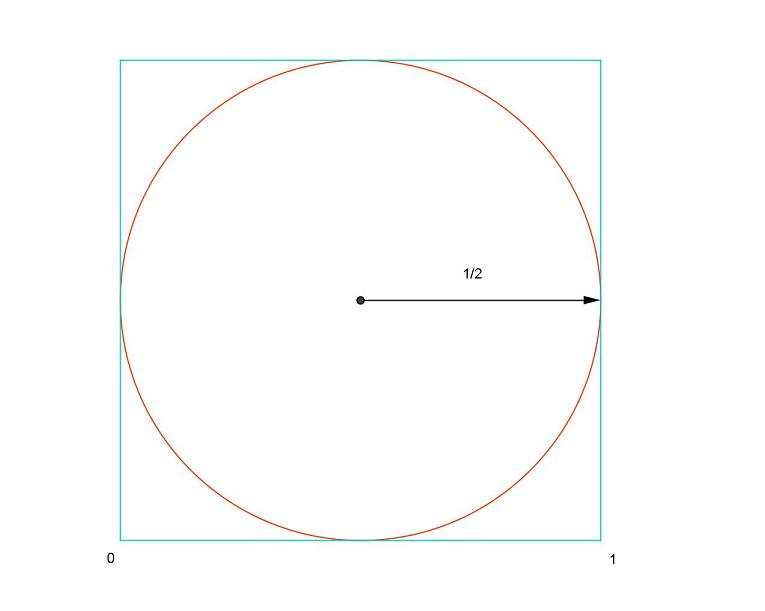
\includegraphics[width=0.5\textwidth]{figure1.jpg}
\caption{Example in dimension $2$.}
\end{figure}

\begin{figure}
\centering
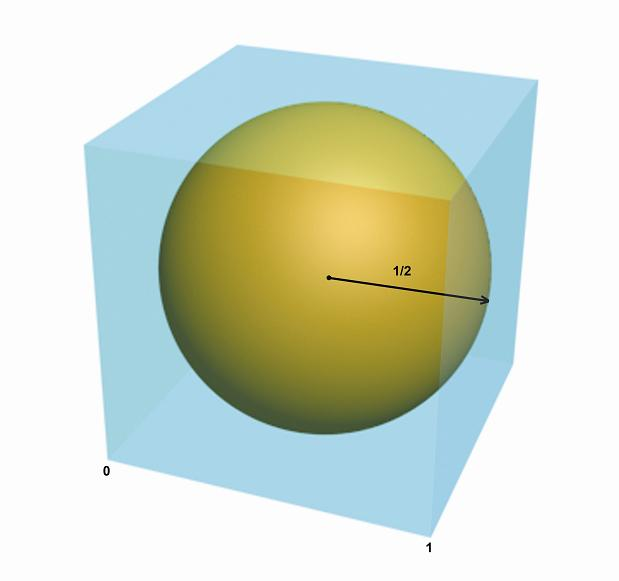
\includegraphics[width=0.5\textwidth]{figure2.jpg}
\caption{Example in dimension $3$.}
\end{figure}

Then, the general case is,
$\dfrac{\text{vol}(B^{n}_{1/2})}{\text{vol}(_{0}^{}\square_{1}^{n})} =
\text{vol}(B_{1/2}^{n}) =$ fraction of unit cube taken up by largest
ball contained inside.

Now, using Stirling's approximation, $\Gamma(x + 1) \approx \sqrt{2
  \pi x}\left(\dfrac{x}{e}\right)^{x}$, $x \in \mathbb{R}_{\geq 0}$,
we have that asymptotically,

$\text{vol}(B_{1/2}^{n})
\stackrel{n \rightarrow \infty}{\longrightarrow}
\dfrac{\pi^{\frac{n}{2}}(\frac{1}{2})^{n}}{\sqrt{2 \pi\frac{n}{2}}(\frac{n/2}{e})^{\frac{n}{2}}} =
\dfrac{\pi ^\frac{n}{2} 2^\frac{n}{2} e^\frac{n}{2}}{\sqrt{\pi n} n^\frac{n}{2} 2^{n}} =
\dfrac{1}{\sqrt{\pi n}}\left( \dfrac{\pi e}{2n} \right)^{\frac{n}{2}} 
\stackrel{n \rightarrow \infty}{\longrightarrow}
0$.

\begin{example} $\dfrac{\text{vol}(B_{1/2}^{100})}{\text{vol}(\square^{100})} \approx 10^{-67}$.
\end{example}

Then, we have bad news for numerical integration (for example in the
case of Monte Carlo integration) when it is used in physics or in
financial mathematics because, by the example above, we will be not
able to count from $1$ to $10^{-67}$. This is too long. So, this works
worst as the dimension increases. In conclusion, we will not use Monte
Carlo Integration to calculate volumes in high dimensions because the
volumes of the balls will be so tiny.

\begin{remark} An example of Monte Carlo Integration in physics
  consists in throw random points into our space and count how many
  points fall inside and how many points fall outside. Then, do the
  fraction which divides the number of points inside and the number of
  points thrown and this fraction approximates the volume (it is used
  at CERN). In the other hand, Monte Carlo Integration is used in
  financial mathematics, for example if we have a portfolio with many
  variables and we have to integrate, one way to integrate by all this
  variables is using Monte Carlo Integration.
\end{remark}


\section{Lattices and lattice polytopes}

Now, we will talk about lattice packings of spheres. A lattice has two
different meanings in mathematics: a partially ordered set or a
group. We are gonna talk about the group.

The most important lattice is $\mathbb{Z}^{d}$, and it's called the
integer lattice. This is an abelian group with the sum: $x, y \in
\mathbb{Z}^{d} \Rightarrow - x \in \mathbb{Z}^{d}, x + y \in
\mathbb{Z}^{d}$, and the sum is commutative.

Now, if we have $v_{1}, \ldots, v_{n} \in \mathbb{Z}^{d}$, and we have
a look to $P = \text{conv}\lbrace v_{1}, \ldots, v_{n} \rbrace
\subseteq \mathbb{R}^{d}$, we define a lattice polytope as the convex
hull of a finite set of points with integer coordinates.

\begin{figure}
\centering
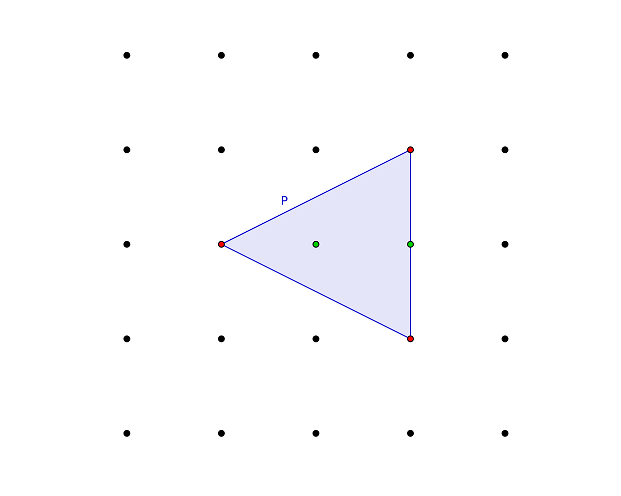
\includegraphics[width=0.5\textwidth]{figure3.png}
\caption{A lattice triangle.}
\end{figure}

Now, we can do the next question: When two lattice triangles "the
same"? The first observation is that we have to answer is: When two
polytopes are "the same"? In Figure 4, we can say that the two lattice
triangles are "the same" because they share all properties respect to
the lattice.

\begin{figure}
\centering
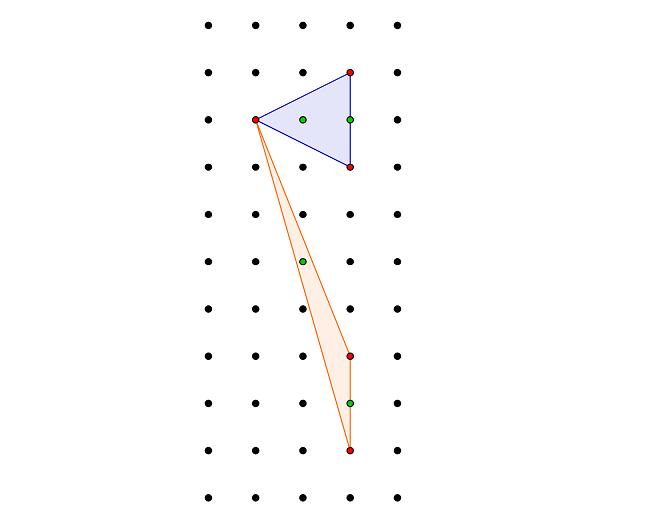
\includegraphics[width=0.5\textwidth]{figure4.png}
\caption{Two lattice triangles.}
\end{figure}

Now, forgetting lattices, the answer to the question for polytopes in
general is: Klein's Erlangen Program. In this program, Klein
identifies the geometry with the groups of automorphisms, i.e., what
Klein makes is to say what the geometry is, by seeing which group of
automorphisms leaves certain object invariant.

Some groups that we must have in mind are $O(n, \mathbb{R}) = \lbrace
A \in \mathbb{R}^{n \times n} : A^{-1} = A^{T} \rbrace$ and $SO(n,
\mathbb{R}) = O(n, \mathbb{R}) \cap \lbrace A \in \mathbb{R}^{n \times
  n} : \det A = 1 \rbrace$. In the other hand, we can also have in
mind the set of translations in $\mathbb{R}^{n \times n}$, $T(n,
\mathbb{R}^{n \times n})$, which satisfies $SO(n, \mathbb{R}^{n \times
  n}) \rtimes T(n, \mathbb{R})$, where $\rtimes$ is the semi-direct
product, which means: two subsets, $P, Q \subseteq \mathbb{R}^{n}$,
are ''the same'' if $\exists A \in O(n)$ and $\exists t \in
\mathbb{R}^{n} : Q = A \cdot P + t$, i.e., I can obtain $Q$ from $P$
through a rotation $A$ and a translation $t$ (i.e., $P$ and $Q$ are
congruent), and this is what we know as Euclidean Geometry.

Now, remembering lattices, we have to change the euclidean geometry by
lattice geometry, i.e., we want bijective homomorphisms that preserves
the lattices. So, we want to determine $\text{Aut}(\mathbb{Z}^{d}) =
\lbrace \text{affine transformations that leave } \mathbb{Z}^{d}
\text{ invariant} \rbrace$, and this is to find conditions on $A \in
\mathbb{R}^{n \times n}$ and $t \in \mathbb{R}^{n}$ such that $Ax + t
\in \mathbb{Z}^{d}$, $\forall x \in \mathbb{Z}^{d}$.
These conditions are:

\begin{itemize}
\item $x = 0$, want $A \cdot 0 + t \in \mathbb{Z}^{d}
  \Longleftrightarrow t \in \mathbb{Z}^{d}$.

\item $x = e_{i}$, with $e_{i}$ a generating vector of our lattice,
  want $A \cdot e_{i} \in \mathbb{Z}^{d} \Longleftrightarrow$ every
  column of $A \in \mathbb{Z}^{d} \Longleftrightarrow A \in
  \mathbb{Z}^{d \times d}$.
\end{itemize}

Now, for $A$ to be an automorphism, it must be invertible, and
$A^{-1}$ must belong to $\mathbb{Z}^{d \times d}$.

\begin{example} Suppose that $d = 2$. We have
  $\left( \begin{smallmatrix} a & b \\ c & d \end{smallmatrix} \right)
  \in \mathbb{Z}^{2 \times 2}$. Then, $A^{-1} = \frac{1}{ad - bc}
  \left( \begin{smallmatrix} d & -b \\ -c & a \end{smallmatrix} \right) =
  \frac{1}{\det A}\left[ (c_{ij}) \right]$, where $(c_{ij})$
  represents the cofactors of $A$. And $A^{-1} \in \mathbb{Z}^{2
    \times 2}$ because $ad - bc$ never divides the entries of
  $\left( \begin{smallmatrix} d & - b \\ - c & a \end{smallmatrix}
  \right)$. (This has to be proved.)
\end{example}

Then, $\text{Aut}(\mathbb{Z}^{d}) = \left\lbrace A \in \mathbb{Z}^{d
    \times d} : \det A = \pm 1 \right\rbrace \rtimes \mathbb{Z}$.

Observe that the set of orientation-preserving linear (not affine)
automorphisms of $\mathbb{Z}^{d}$ is $\Sl_d(\ZZ) = \big\{ A \in
\mathbb{Z}^{d \times d} : \det A = 1 \}$, the special linear group
with integer coefficients. On the other hand, $\left\lbrace A \in
  \mathbb{Z}^{d \times d} : \det A = -1 \right\rbrace$ is not a group.

  Then, what lattice geometry means is that geometry with group
  automorphisms: $Sl_{d}(\mathbb{Z}) \rtimes \mathbb{Z}^{d}$, and this
  is mapping $x \longmapsto Ax + t$, with $t \in \mathbb{Z}^{d}$, $A
  \in \mathbb{Z}^{d \times d}$, and $\det A = \pm 1$. Then, any two
  lattice polytopes in correspondence by any of this automorphisms
  will be the same polytope.

  Now, observe that in Figure 4, using that the image of the vectors
  are the same than the columns of the matrix $A$, we have that $A =
  \left[ \begin{smallmatrix} 1 & 0 \\ -2 & 1 \end{smallmatrix}
  \right]$, with $A \cdot e_{1} = \left( \begin{smallmatrix} 1 \\ -
      2 \end{smallmatrix}
  \right)$ and $A \cdot e_{2} = \left( \begin{smallmatrix} 0 \\
      1 \end{smallmatrix} \right)$.  Also, observe that the following
  transforms (called \emph{shears}) are typical lattice transforms in
  $\mathbb{Z}^{2}$: $\left[ \begin{smallmatrix} 1 & 0 \\ * &
      1 \end{smallmatrix} \right]$ and $\left[ \begin{smallmatrix} 1 &
      * \\ 0 & 1 \end{smallmatrix} \right]$. This can be used in
  exercise 3 of list 1.

After seen this, we are going to see some definitions:

Let $P \subseteq \mathbb{R}^{d}$ be a polytope ($\sim$ convex hull of
finitely many points). A linear inequality of the form $ax \leq b$
with $a \in (\mathbb{R}^{d})^{*}$, $x \in \mathbb{R}^{d}$, $b \in
\mathbb{R}$ is valid for $P$ if all points of $P$ satisfy it. (observe
that $(\mathbb{R}^{d})^{*}$ represents the dual space of
$\mathbb{R}^{d}$).

A face of $P$ is $P \cap \lbrace x \in \mathbb{R}^{d} : ax = b
\rbrace$, where $ax \leqslant b$ is a valid linear inequality for
$P$. In particular, $\emptyset$ is always a face of $P$ (example: $0x
\leqslant 1$), and $P$ is always a face of $P$ (example: $0x \leqslant
0$). This, bring us to a second meaning of lattice:

The face lattice of $P$ is the poset (partially ordered set) of faces
of $P$ with the inclusion.

\begin{example} If we have the polytope of figure 5, this polytope
  will have the face lattice of figure 6 (where O represents the
  $\emptyset$).
\end{example}

\begin{figure}
\centering
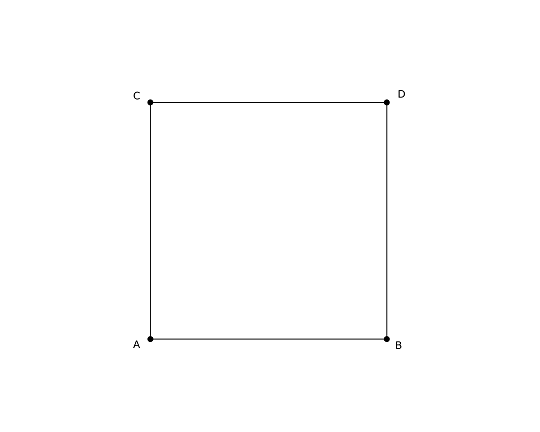
\includegraphics[width=0.5\textwidth]{figure5.png}
\caption{Square ABCD.}
\end{figure}

\begin{figure}
\centering
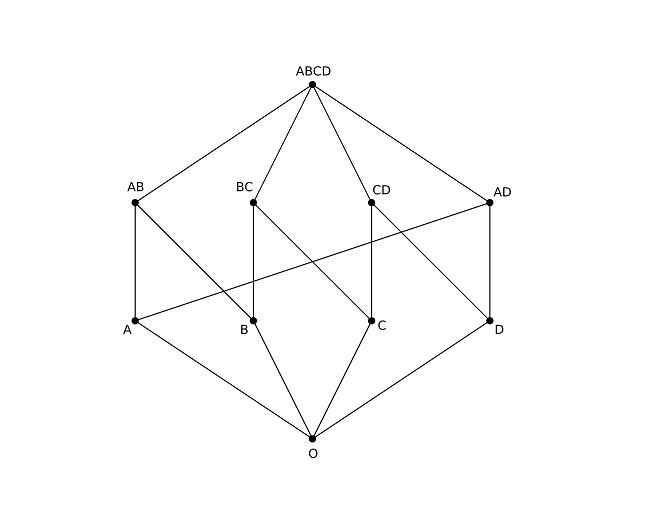
\includegraphics[width=0.5\textwidth]{figure6.png}
\caption{Its face lattice.}
\end{figure}


If anybody wants to read about this, then read ''Lectures on
Polytopes'' by Ziegler.

This can be applied to cubes, for example, as follows:

\begin{center}
  $(1 0 0 0 1 1)\left( \begin{array}{c} x_{1} \\ x_{2} \\ x_{3} \\
      x_{4} \\ x_{5} \\ x_{6} \end{array} \right) \leqslant k$,
\end{center}

where $k$ represents the non-zero entries (in this case $k = 3$), and
using this, we can calculate the barycenters.


% Local Variables: 
% mode: latex
% TeX-master: "dag-2011"
% End: 
 

\bibliographystyle{amsalpha}
\bibliography{dag}

\end{document}

%%% Local Variables: 
%%% mode: latex
%%% TeX-master: t
%%% End: 
